\documentclass[a4paper,10pt]{article}
\usepackage[polish]{babel}
\usepackage[utf8]{inputenc}
\usepackage{polski}
\usepackage[T1]{fontenc}
%\usepackage{enumerate}
\usepackage{indentfirst}
\usepackage{graphicx}
\usepackage{fancyhdr}

\author{Mateusz Gałażyn, Jeremi Niedziela}
\title{Krótki kurs tworzenia stron w technologii PHP}
\setlength{\textheight}{24cm}
\setlength{\textwidth}{15.92cm}
\setlength{\footskip}{10mm}
\setlength{\oddsidemargin}{0mm}
\setlength{\evensidemargin}{0mm}
\setlength{\topmargin}{0mm}
\setlength{\headsep}{5mm}


\frenchspacing
\begin{document}

\pagestyle{fancy}
%\rhead{Prawa strona nagłówka. Strona nr \thepage}
\lhead{Krótki kurs tworzenia stron w technologii PHP}


\maketitle
\section{Wstęp}
Ten krótki kurs ma na celu przedstawienie sposobu pisania stron w przy użyciu technologii Apache + MySQL + PHP (w skrócie AMP) - jednego z najpopularniejszych zestawów oprogramowania służącego do uruchamiania serwisów WWW. 
\subsection{Mechanizm działania systemu AMP} 
Gdy użytkownik strony uruchamia przeglądarkę i wpisuje w pasek adresu, adres szukanego serwisu WWW, przeglądarka nawiązuje połączenie z serwerem na którym są uruchomione usługi umożliwiające dostęp do strony. \\
\textbf{Apache} - jest to najszerzej stosowany w internecie serwer HTTP \\
\textbf{PHP} - jeden z najpopularniejszych języków programowania używany do tworzenia stron WWW. \\
\textbf{MySQL} - system zarządzania bazami danych za pomocą języka SQL \\
Schemat połączeń jest przedstawiony na ilustracji poniżej:

\begin{center}
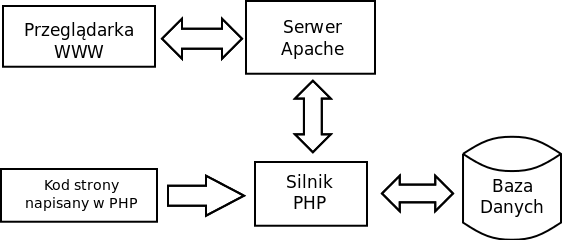
\includegraphics[width=0.7\textwidth]{LAMP.png} 
\end{center}

Żądanie otrzymane od przeglądarki jest przechwytywane przez serwer Apache, który przetwarzając je uruchamia kod strony napisany w języku PHP. Następnie silnik PHP po komunikuje się z bazą danych, pobiera dane, przetwarza je i zamienia na kod HTML, który zwraca serwerowi Apache. W kolejnym kroku serwer Apache wysyła kod HTML razem z obrazami umieszczonymi na stronie i stylami do przeglądarki, która renderuje i wyświetla stronę.

\section{Instalacja środowiska AMP}
\subsection{Instalacja na systemie Windows}
\subsubsection{Instalacja serwera Apache}
\subsubsection{Instalacja PHP}
\subsubsection{Instalacja serwera MySQL}
\subsection{Instalacja na systemie Linux}
\subsubsection{Instalacja serwera Apache}
\subsubsection{Instalacja PHP}
\subsubsection{Instalacja serwera MySQL}
\subsection{Konfiguracja}
\subsubsection{Konfiguracja Apache}
\subsubsection{Konfiguracja PHP}
\subsubsection{Konfiguracja MySQL}
\section{Projekt forum dyskusyjnego}
Naszym celem jest jest zbudowanie prostego forum dyskusyjnego. Musimy dać możliwość rejestrowania się poszczególnym użytkownikom, dodawania własnych wątków oraz odpowiadania na już utworzone. Potrzebne będzie też konto administratora, który będzie miał prawo moderacji postów już utworzonych.
\subsection{Układ podstron}
Gdy zostanie już ustalona lista wymaganych funkcjonalności projektowanego serwisu, następnym etapem jest stworzenie układu poszczególnych podstron.
\paragraph{Strona główna} Tutaj trzeba wyświetlić listę tematów (wraz z odnośnikami do podstrony, na którym będzie pojedynczy wątek wyświetlany w całości) które zostały założone na forum, umieścić odnośniki do podstrony z formularzem używanym do zalogowania się i rejestracji dla użytkowników oraz odnośnik do podstrony umożliwiającej założenie nowego tematu.
\paragraph{Podstrona wątku} W tym miejscu trzeba wyświetlić wszystkie posty w danym wątku, oraz formularz dający możliwość odpowiedzi w tym wątku. Gdy administrator wejdzie na tą podstronę, trzeba dać także dodatkowe możliwości edycji i usuwania poszczególnych postów.
\paragraph{Podstrona logowania} Zawierać będzie formularz logowania umożliwiający uwierzytelnienie użytkownika wchodzącego stronę. Uwierzytelnienie będzie polegało na porównaniu nazwy użytkownika i hasła z obecnymi w bazie danych. Po zalogowaniu się, użytkownik zostanie przekierowany z powrotem na stronę główną. Podstrona dostępna tylko dla niezalogowanych użytkowników.
\paragraph{Podstrona rejestracji} Odpowiedzialna za obsługę rejestracji nowego użytkownika. Trzeba będzie wyświetlić formularz rejestracji, odebrać i zweryfikować dane oraz dodać je do bazy danych.

\paragraph{Podstrona nowego wątku} Podstrona z formularzem umożliwiającym dodanie nowego wątku. Po odebraniu danych od użytkownika trzeba będzie dokonać ich weryfikacji i dodać do bazy danych. Na koniec trzeba przekierować użytkownika do podstrony wątku.

\paragraph{Podstrona edycji postu} Podstrona z formularzem umożliwiającym edycję własnych postów, a także w przypadku administratora - edycji każdego postu. Przekierowuje z powrotem do podstrony wyświetlającej cały wątek.

\subsection{Projekt bazy danych}

\section{Kod strony}

\end{document}
